
\section{Multivariate analysis}
\label{sec:mva}

At the end of the cut-based analysis,
combining the three categories,
we obtain a signal significance of $S/\sqrt{B}\simeq 1.7 (3.5)$
with all backgrounds (only QCD $4b$) taken into account.
%
We now show how this signal significance
 can be enhanced when the cut-based analysis
 is complemented with a multivariate analysis (MVA).
%
 Multivariate techniques are by now a mature tool
 in high-energy physics data analysis, opening
 new avenues for improving the performance
of many measurements and searches at high-energy colliders.
%
In particular, the classification of events between signal and
background processes by means of MVAs is a
commonly applied strategy in LHC
applications~\cite{Baldi:2014pta,Aaltonen:2012qt,
  Wardrope:2014kya,Chatrchyan:2013zna,Dall'Osso:2015aia}.

In this section, first of all we present the specific MVA that we use,
based on feed-forward multi-layer neural networks.
%
We then introduce the input variables that are
used in the MVA, including the jet substructure
variables, and then present the signal significance obtained
by applying the MVA.
%
Then we assess the robustness of the MVA strategy in
high-PU environments.

\subsection{Deep artificial neural networks}

%
The specific type of  MVA that we use to
disentangle signal and background events is
a multi-layer feed-forward artificial neural network (ANN),
known as a {\it perceptron}.\footnote{This type of ANNs are the same
  as those used to parametrize Parton Distribution Functions
in the NNPDF global analyses~\cite{DelDebbio:2004qj,Ball:2008by,Ball:2011mu,Ball:2010de}.}
%
This family of ANNs is also known as {\it deep} neural networks, since they have
a richer architecture with hidden layers.
%
The input to the MVA are the
signal and background
events which satisfy the requirements of the
cut-based analysis.
%
The output of the trained ANNs allows the identification, in a fully automated way,
of the most relevant variables to discriminate between 
signal and background.

In this work, the ANN that we use has the following architecture.
\be
\label{eq:nn1}
N_{\mathrm{var}}\times5\times3\times1 \, ,
\ee
where $N_{\mathrm{var}}$ represents the number of input variables for the MVA,
which is different in the resolved, intermediate, and boosted categories.
%
All neural-network layers use a sigmoid activation function, allowing
for a probabilistic
interpretation of the ANN output.
%
In Fig.~\ref{fig:nnarch} we show an illustrative
example of a ANN used in this work, corresponding 
to the case of the boosted category (thus $N_{\mathrm{var}}=21$, as we explain below).

%%%%%%%%%%%%%%%%%%%%%%%%
\begin{figure}[t]
  \begin{center}
      \vspace{-1cm}
  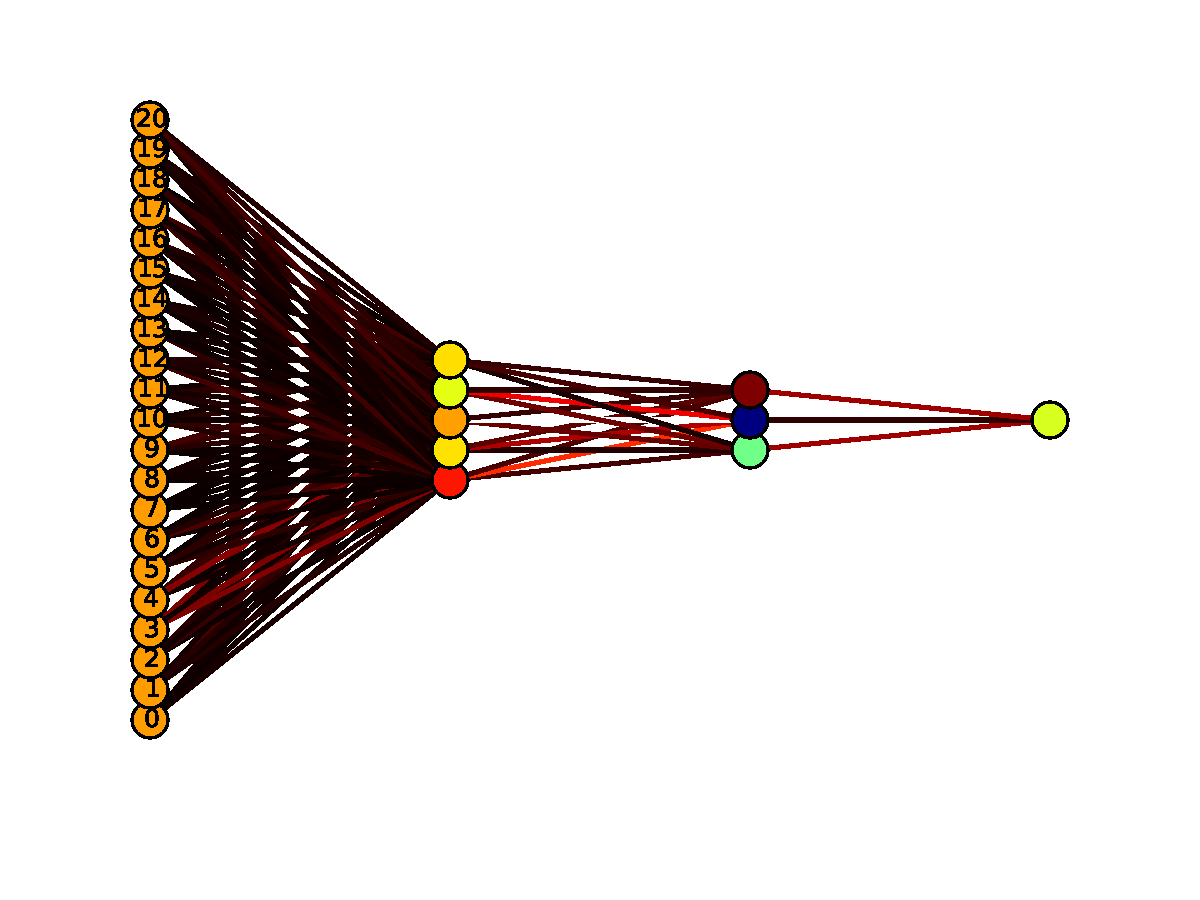
\includegraphics[width=0.90\textwidth]{plots/bst_nnarch_noPU.pdf}
  \vspace{-2cm}
  \caption{\small Architecture of the Artificial
    Neural Network (ANN)
    used for the analysis of the
    boosted
    category, with $N_{\rm var}=21$ input variables and thus
    the same number of neurons
  in the first layer.
  %
  The color code in the neuron connections (the weights) is a heat map obtained
  at the end of the GA training,
  with red indicating larger values and black indicating smaller values.
}
\label{fig:nnarch}
\end{center}
\end{figure}
%%%%%%%%%%%%%%%%%%%%%%%

The training of the ANN for the signal/background classification task
proceeds as follows.
%
Given a set of $N_{\mathrm{var}}$  kinematic variables $\{k\}_i$ associated with the event $i$, and a set of neural network weight
parameters $\{\omega\}$, we interpret the neural network output $y_i$
(the activation state of the
neuron in the last layer)
as the probability that the event $i$ originates from the signal process,
\be
y_i = P(y^\prime_i=1|\{k\}_i, \{\omega\} )\, ,
\ee
where $y_i^\prime$ represents the true classification of the event $i$, {\it i.e},
$y^\prime = 1$ for signal and $y^\prime = 0$ for background events.
%
With this interpretation, our general classification probability including background events is given by
\be
P(y_i^\prime|\{k\}_i, \{\omega\}) = y_i^{y^\prime_i}(1-y_i)^{1-y^\prime_i} \, ,
\ee
which implies that the  error function $E(\{\omega\})$
that needs to be minimized during the ANN training is 
the cross-entropy function, defined as
 \bea
 &&E(\{\omega\}) \equiv -\log\left(\prod_i^{N_{\text{ev}}} P(y_i^\prime|\{k\}_i, \{\omega\})\right)\nonumber\\
 &&=
 \sum_i^{N_{\text{ev}}} \lc y^\prime_i\log{y_i} + (1-y^\prime_i)\log{(1-y_i)}\rc \, ,
 \label{cross-entropy}
 \eea
 where $N_{\text{ev}}$ is the number of
 Monte Carlo events that are used for the ANN training.
 %
 The ANN is trained both on the signal and background MC events,
 so it is crucial to ensure that the input MC sample is large enough
 to avoid the contamination from MC statistical fluctuations.

 
 The training of the neural networks thus consist on the
 minimization of the cross-entropy error,
 Eq.~(\ref{cross-entropy}), which in this work is achieved using a
 Genetic Algorithm (GA).
 %
 Genetic Algorithms~\cite{quevedo,tau,Abel:2014xta,Nesseris:2012tt} are
 non-deterministic
 minimization strategies suitable for the solution
 of complex optimization problems, for instance when a very large number
 of quasi-equivalent minima are present.
 %
 GAs are inspired on natural selection processes
 that emulate biological evolution. 
 %
 In our case, the GA training is performed for a very large 
 number of generations, $N_{\rm gen}=5\cdot 10^{4}$, to avoid the risk of
 under-training.
 %
 We have verified that if a much larger number of generations
 are used, the results are unchanged.
 %

 In order to avoid over-fitting,
 we have used a cross-validation stopping
 criterion, in particular the same one as
 that used in the NNPDF3.0 analysis~\cite{Ball:2014uwa}.
 %
 This cross-validation entails dividing the input MC dataset into two disjoint sets,
 and use one for the training and the other for the validation: the optimal
 stopping point is then indicated by the minimum of the error function
 Eq.~(\ref{cross-entropy}) for the validation sub-sample.
 %
 This indicates the point where we are training on the statistical fluctuations
 of the input MC samples, rather than in the underlying (smooth) physical
 distributions.
 

 \subsection{Input kinematical variables}
 \label{sec:input}

 To ensure that we include the variables with higher discriminatory power,
 we need to train
 the MVA on a large number of kinematic distributions.
%
In this work we use different sets of
input variables for the three categories.
%
In particular, in the case of large-$R$ jets (for the boosted
and intermediate categories), we are fully exploiting the jet
substructure information.

For the three categories, boosted, intermediate and resolved,
the following common variables are used as input to the MVA:
\begin{itemize}
\item The transverse momenta of the leading and subleading Higgs, $p_{T,h_1}$ and $p_{T,h_2}$.
\item The transverse momentum of the reconstructed Higgs pair, $p_{T,hh}$.
\item The invariant masses of the leading and sub-leading Higgs candidates, $m_{h,1}$ and $m_{h,2}$.
\item The invariant mass of the reconstructed Higgs pair, $m_{hh}$.
\item The separation in the $\phi$--$\eta$ plane
  between the two Higgs candidates, $\Delta R_{hh}$.
  \item The separation in $\eta$  between the two Higgs candidates, $\Delta \eta_{hh}$.
\item The separation in $\phi$  between the two Higgs candidates, $\Delta \phi_{hh}$.
\end{itemize}
In addition, in the boosted category we use
  the transverse momenta of the leading, $p_{T,h_{1,1}}$ and $p_{T,h_{1,2}}$ and
  sub-leading, $p_{T,h_{2,1}}$ and $p_{T,h_{2,2}}$, Higgs candidate AKT03 subjets.
  %
  In the resolved category instead,
  the corresponding variables are
  the transverse momenta $p_{T,i}$ of the four leading 
  $b$-tagged small-$R$ jets in the event.
  %
  In the intermediate category, we use the
  transverse momenta of the subjets
  from the large-$R$ jet $p_{T,h_{1,1}}$ and $p_{T,h_{1,2}}$ and the
 transverse momenta $p_{T,i}$ of the two leading 
  $b$-tagged small-$R$ jets.
  %
 Therefore, we have 13 variables which are common to the three categories.

 In the boosted and intermediate categories, we also include the jet substructure
 variables introduced in Sect.~\ref{sec:analysis} for the
 large-$R$ jets: the $k_t$ splitting scales
 $\sqrt{d_{12}}$, the ratio of 2-to-1 subjettiness $\tau_{12}$,
 and the ratios of energy correlation functions $C^{(\beta)}_2$ and
 $D_2^{(\beta)}$.
 %
 Therefore, we end up with
 a total of $N_{\mathrm{var}}=13,17$ and 21 variables for the
resolved, intermediate, and boosted categories, respectively.


Given that the MVA is able to identify the most discriminatory variables
in an automated way,
and to ignore those that have little effect, it is advantageous to
include as many input variables as possible.
%
This is one of the main advantages of ANNs in this context: they are
inherently redundant, so
adding additional information, even if carries very little weight,
should not degrade
the classification power of the MVA, other than making the GA
minimization somewhat less efficient.

\subsection{MVA results}
\label{sec:signalsignificance}

We now present the results of the MVA, first without PU, and then
later including the effects of PU.
%
First of all, in Fig.~\ref{fig:nnresponse} we show the distribution of
the ANN output at the end of the GA minimization, for the exclusive
boosted, intermediate and resolved categories.
%
All distributions are normalized so that their integral
  adds up to one.
%
The  separation between signal and background is achieved by introducing
a cut, $y_{\rm cut}$, on the ANN output, so that MC events with $y_i\ge
y_{\rm cut}$ are classified as signal events, and those with
 $y_i <
y_{\rm cut}$ as background events.
%
Therefore,
the more differentiated is the distribution of the ANN output
for signal and background events, the more efficient
the MVA discrimination will be.

%%%%%%%%%%%%%%%%%%%%%%%%%%%%
\begin{figure}[t]
\begin{center}
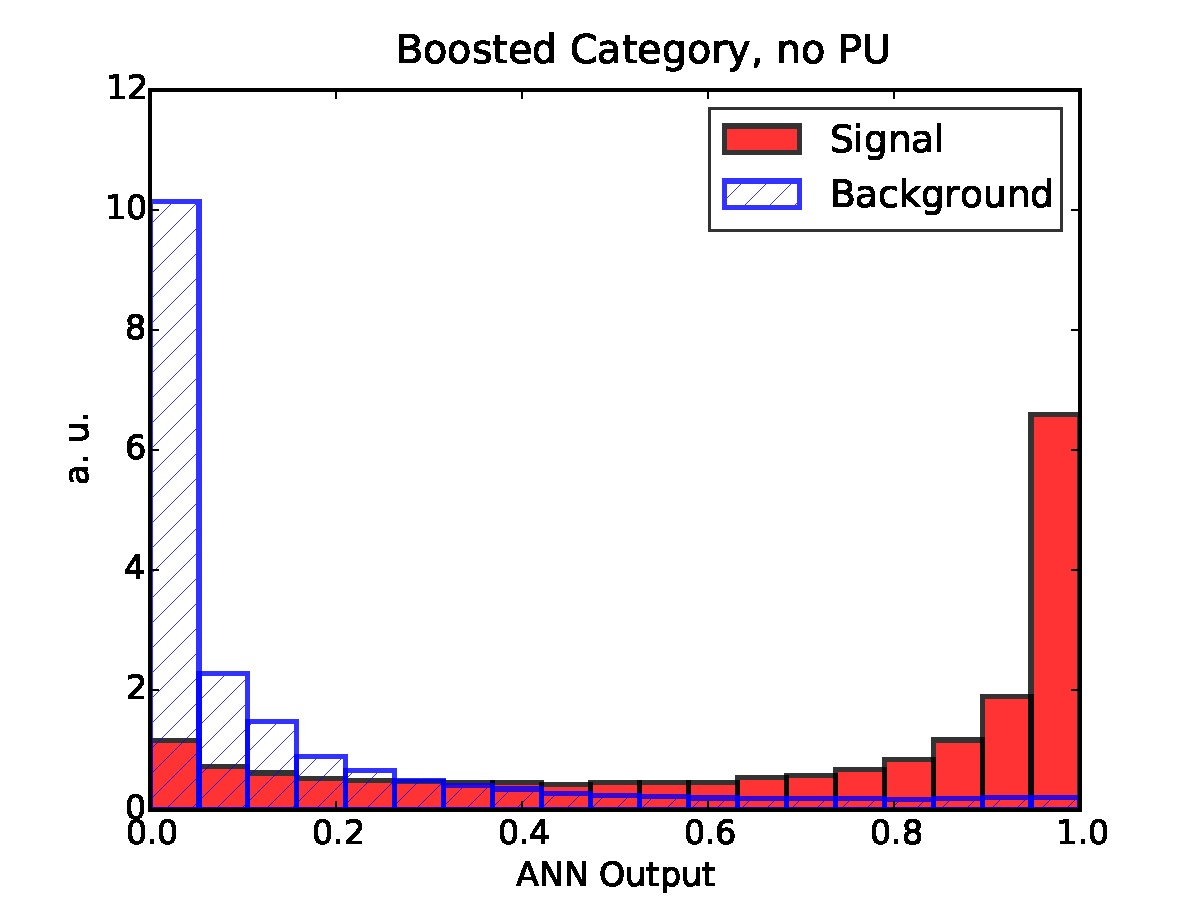
\includegraphics[width=0.65\textwidth]{plots/Boosted_disc_noPU.pdf}
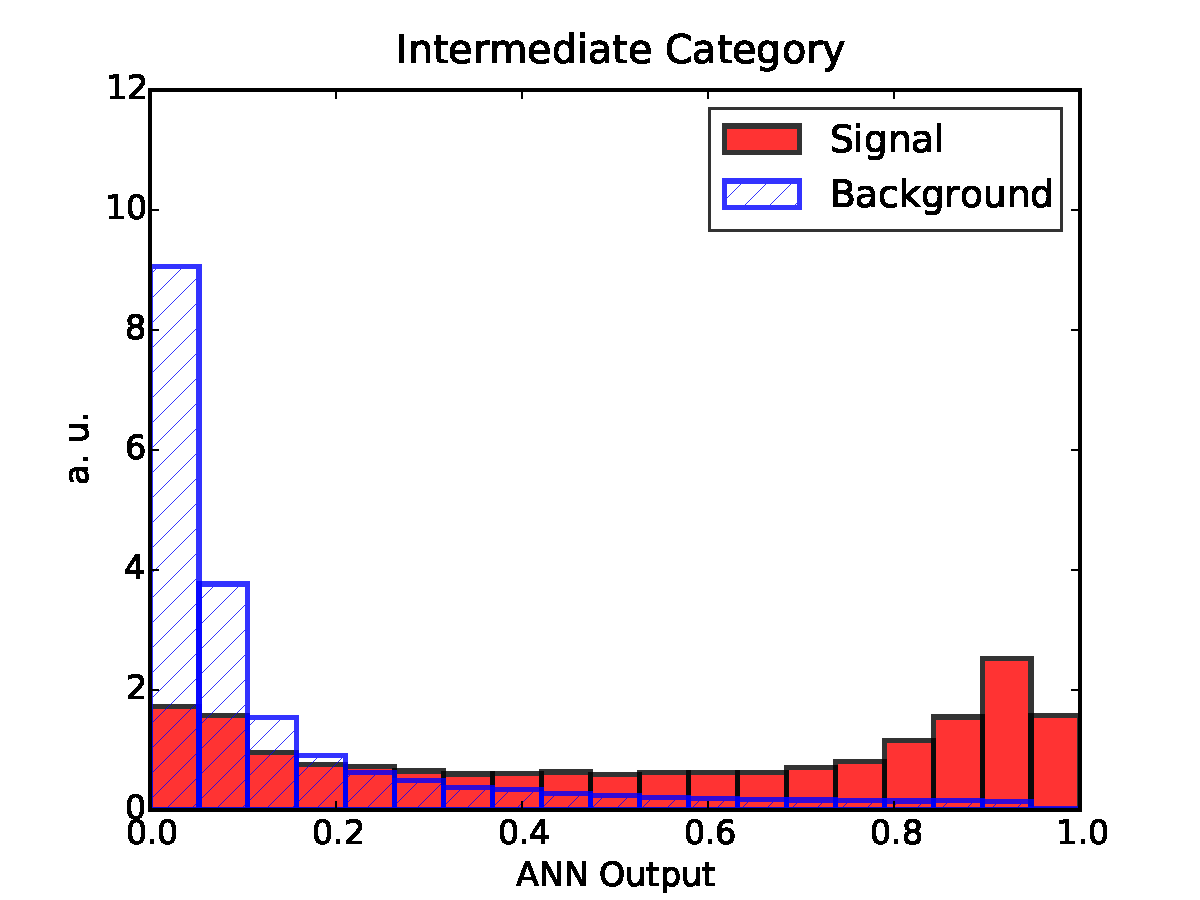
\includegraphics[width=0.48\textwidth]{plots/Intermediate_disc_noPU.pdf}
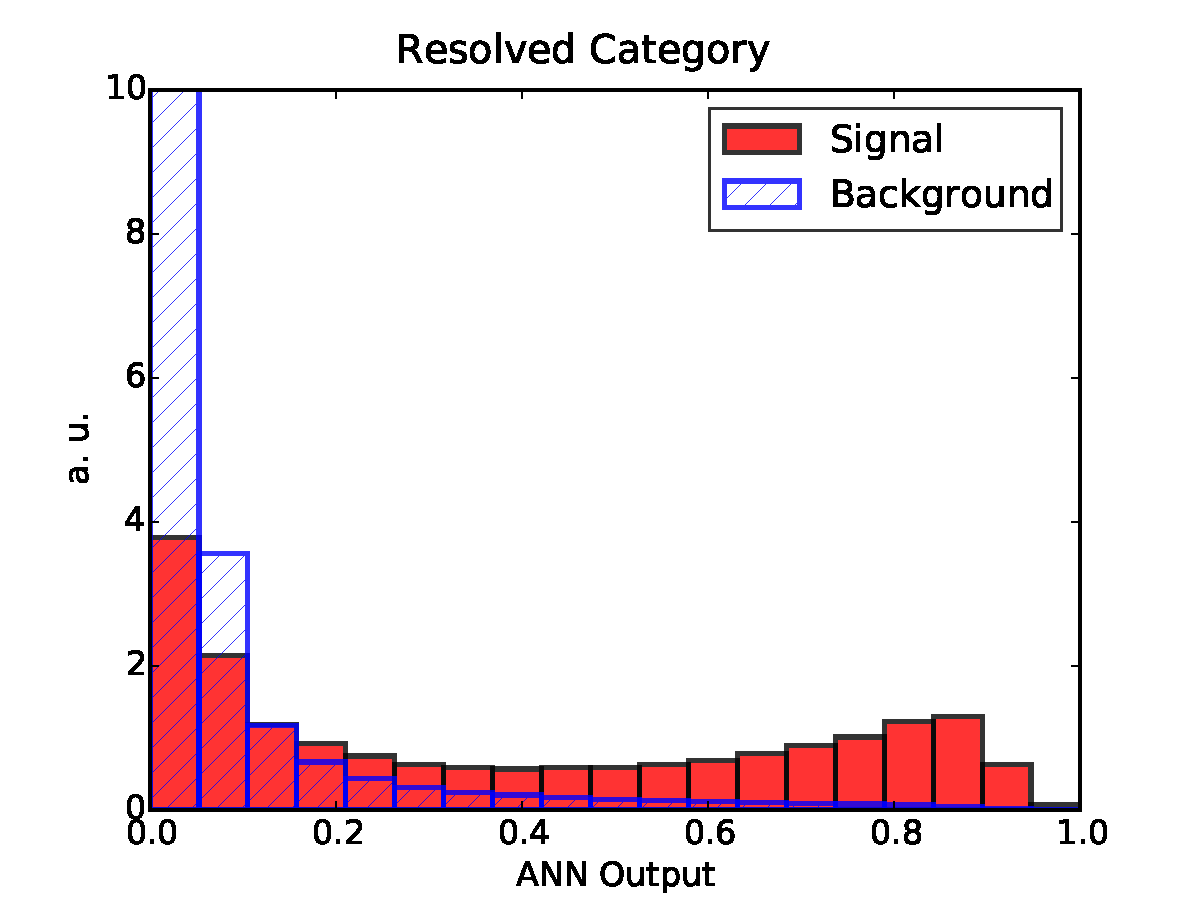
\includegraphics[width=0.48\textwidth]{plots/Resolved_disc_noPU.pdf}
\caption{\small The distributions, at the end of the
  GA training, 
  for the signal and background MC events in the three categories:
  boosted (upper plot), intermediate (lower left plot) and
  resolved (lower right plot), as a function of the ANN output.
}
\label{fig:nnresponse}
\end{center}
\end{figure}
%%%%%%%%%%%%%%%%%%%%%%%

From Fig.~\ref{fig:nnresponse} we see that in the boosted category the MVA manages
to achieve a clear discrimination between signal and background, with the two distributions
nicely peaking at 1 and at 0 respectively.
%
This indicates that introducing a suitable cut
$y_{\rm cut}$
in the ANN output will substantially reduce the background,
while keeping a reasonable signal efficiency.
%
The performance of the MVA discrimination is similar though slightly worse in the intermediate
and resolved categories.
%
The results for the signal selection efficiency and the 
background rejection rate as a function of the cut in the ANN output
$y_{\rm cut}$
define the so-called  Receiver-Operating Characteristic (ROC)
curve, shown in Fig.~\ref{fig:exampleroc}.
%
It is clear that we can achieve  high signal efficiency by using
a small value of $y_{\rm cut}$, but this choice will be
affected from a poor background
rejection.
%
Conversely, using a higher value of the cut will increase background rejection at the
cost of dropping signal efficiency.
%
As could already be inferred from the distribution of neural
networks output in Fig.~\ref{fig:nnresponse}, we find
that our MVA is reasonably efficient
in discriminating signal over background.
%
The performance is best in the case of the boosted category,
and then slightly worse in the resolved
and intermediate categories, consistent with the distributions of
the ANN outputs from
Fig.~\ref{fig:nnresponse}.
%

%%%%%%%%%%%%%%%%%%%%%%%%%%%%%%%%%%%%%%%%%%%%%%
\begin{figure}[t]
\begin{center}
  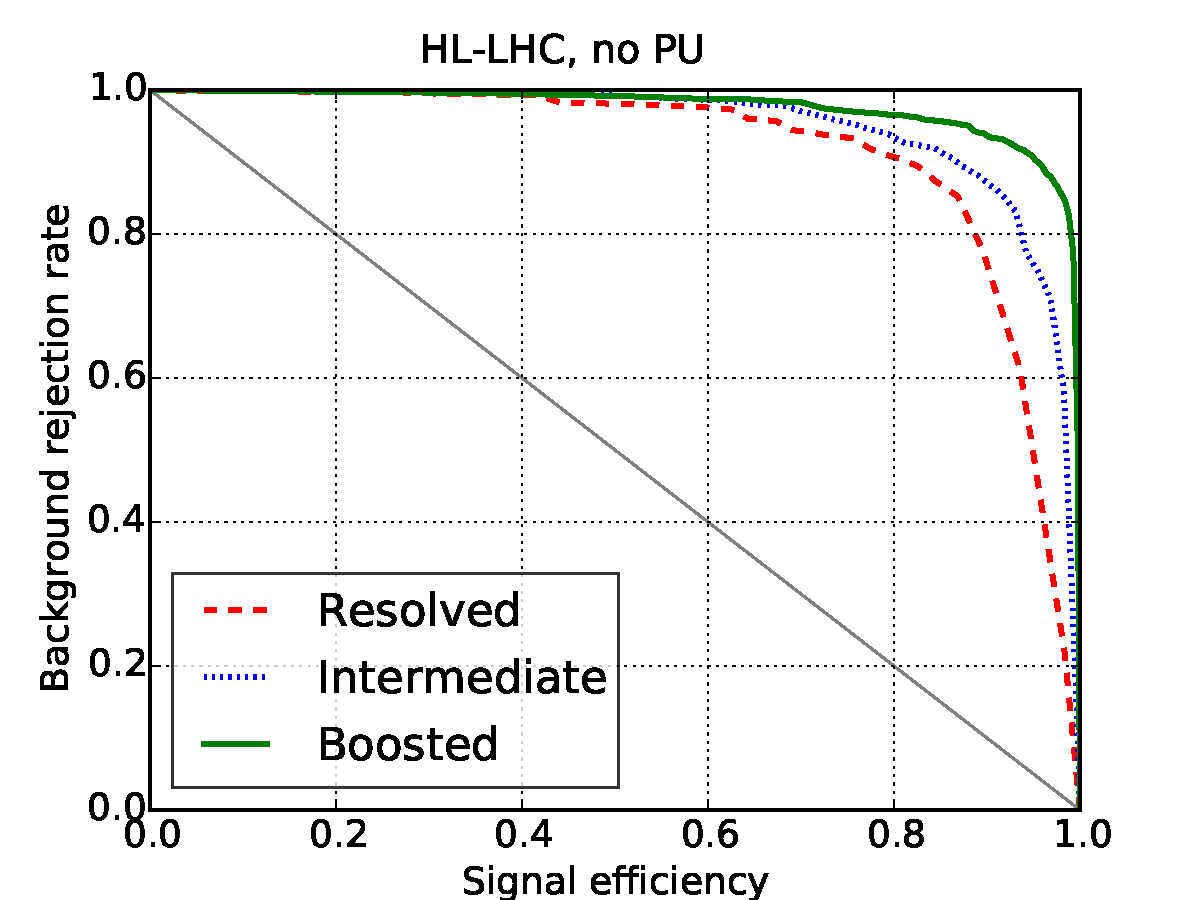
\includegraphics[width=0.49\textwidth]{plots/roc_noPU.pdf}
  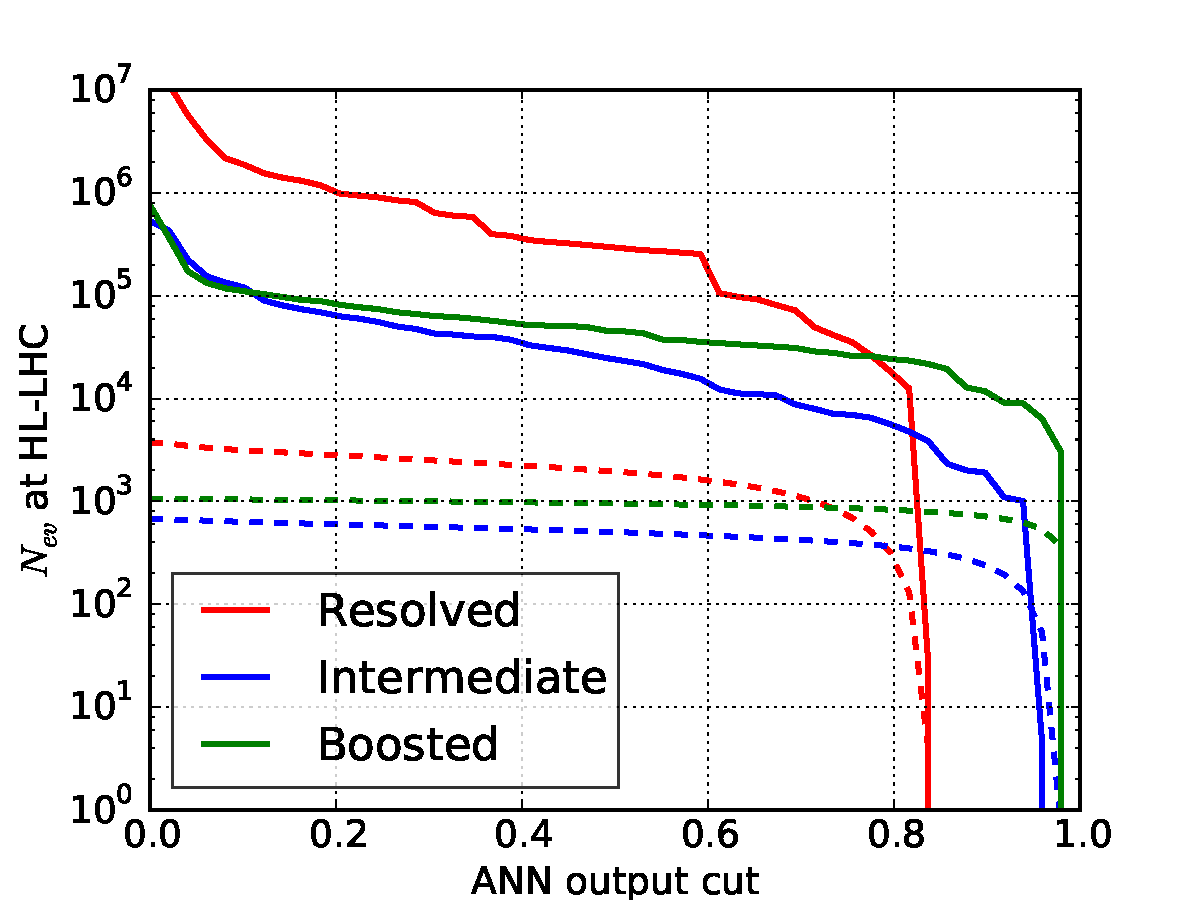
\includegraphics[width=0.49\textwidth]{plots/nev2_noPU.pdf}
\caption{\small Left: ROC curve for the background rejection rate as a function of the signal
  selection efficiency, as the cut $y_{\rm cut}$
  in the ANN output is varied.
  %
  Right: Number of signal (dashed) and background (solid)
  events expected at the HL-LHC as a function of the $y_{\rm cut}$.
}
\label{fig:exampleroc}
\label{fig:nev2}
\end{center}
\end{figure}
%%%%%%%%%%%%%%%%%%%%%%%%%%%%%%%%%%%%%


It important to verify, for each value of
the cut in the ANN output $y_{\rm cut}$, how many
signal and background events are expected at the HL-LHC,
with an integrated luminosity of $\mathcal{L}=3$ ab$^{-1}$.
%
This comparison is shown in 
Fig.~\ref{fig:nev2}.
%
We observe that
in the boosted category, for a value $y_{\rm cut}\simeq 0.8$
we end up with 800 signal events and around $2\cdot 10^4$ background
events.
%
Similar results are obtained in the intermediate and resolved
categories: in the former we find 700 ($6\cdot 10^3$) signal (background)
events for $y_{\rm cut}\simeq 0.8$, and in the latter
1300 ($8\cdot 10^4$) signal (background) events for
$y_{\rm cut}\simeq 0.65$.
%
Note that the MVA achieves a very substantial background suppression
with only a
moderate reduction of signal efficiency.


A useful property of MVAs, as the one used in our
analysis,
is that they provide direct  physical insight about which of the
input variables contribute the most to the separation between
signal and background.
%
In the case of ANNs, this can be quantified by computing the sum
of the absolute value of all the weights connected to a given
input neuron $i$, that is
\be
\label{eq:totweight}
\omega^{\rm (tot)}_i \equiv \sum_{k=1}^{n^{(2)}} \Big|\omega^{(2)}_{ki}\Big| \, ,
\qquad i=1,\ldots,N_{\rm var} \, ,
\ee
with $\omega^{(2)}_{ki}$ the value of the weight connecting
the $k$-th neutron of the second layer with the $i$-th neuron of
the first (input) layer, and $n^{(2)}=5$ the number of
neurons in the second layer.
%
Those input variables with a larger value of $\omega^{\rm (tot)}_i$ will be those
that play a dominant role in enhancing the signal
discrimination using the MVA.


%%%%%%%%%%%%%%%%%%%%%%%%
\begin{figure}[t]
  \begin{center}
    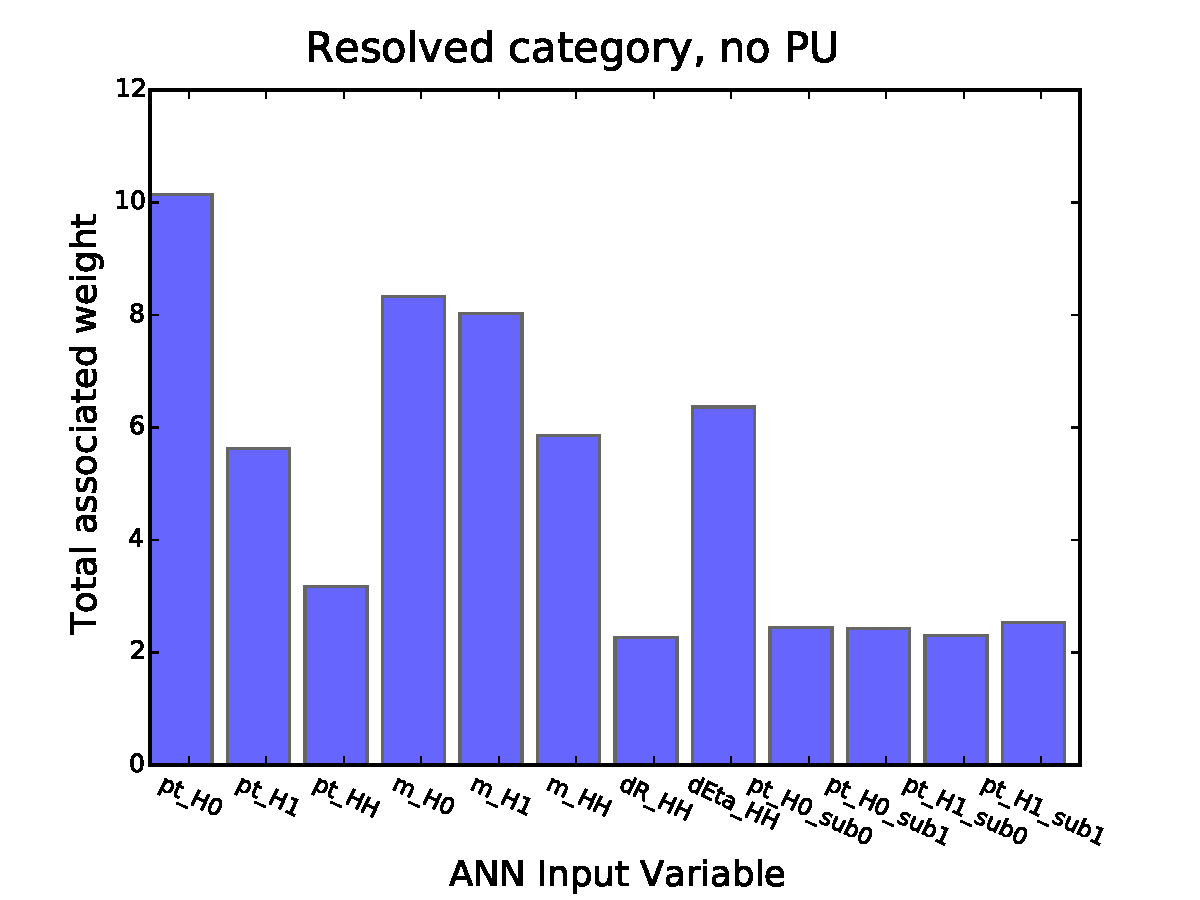
\includegraphics[width=0.49\textwidth]{plots/res_wgthist_noPU.pdf}
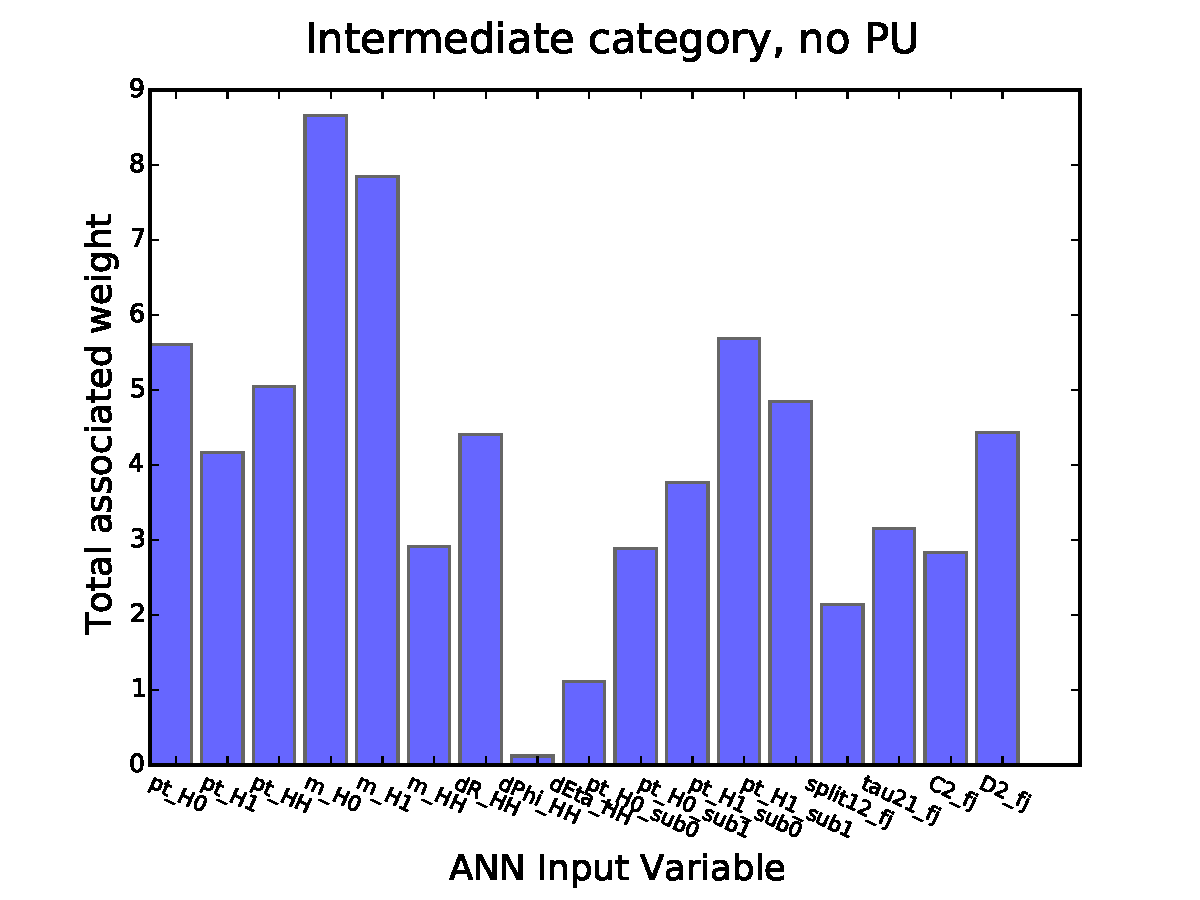
\includegraphics[width=0.49\textwidth]{plots/int_wgthist_noPU.pdf}
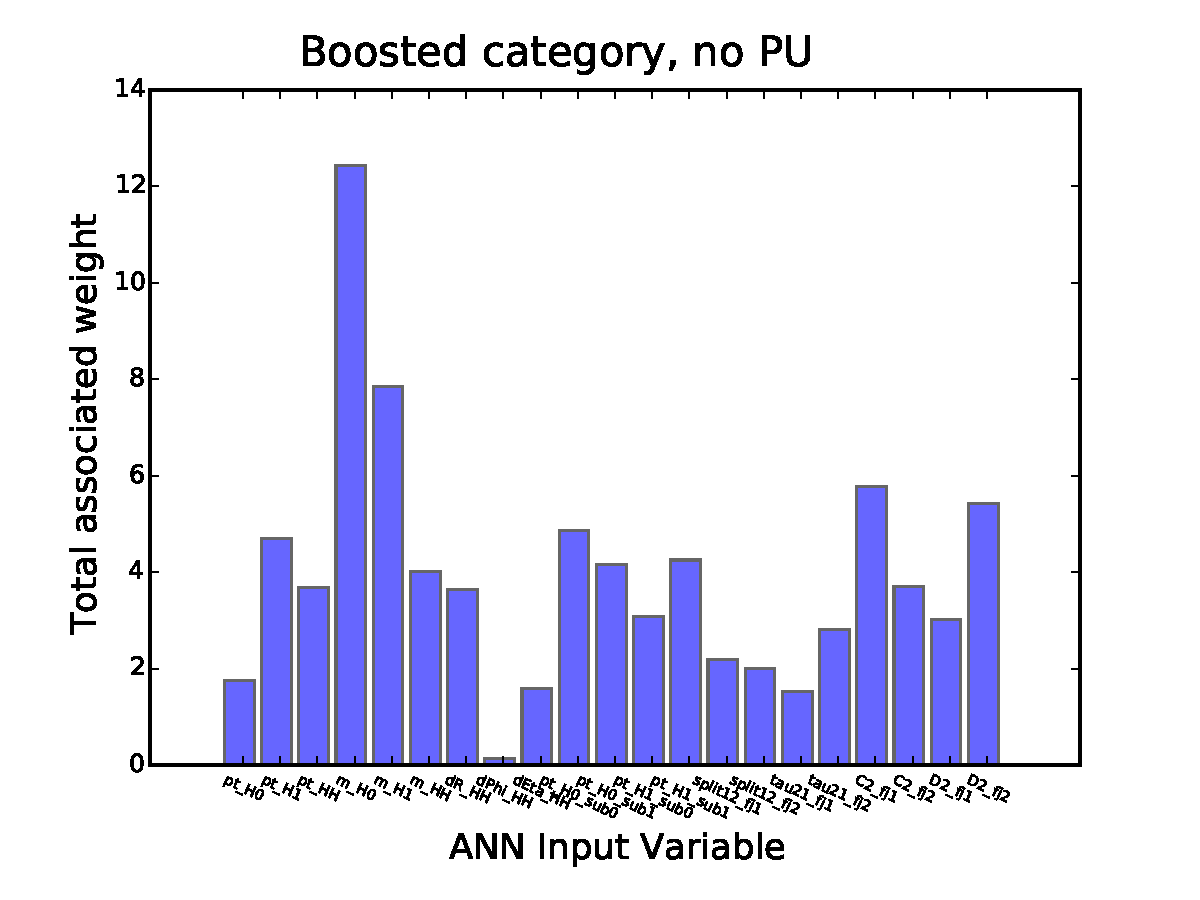
\includegraphics[width=0.75\textwidth]{plots/bst_wgthist_noPU.pdf}
\vspace{-0.5cm}
\caption{\small
Distribution of the total associated weight,
Eq.~(\ref{eq:totweight}) for each of the $N_{\rm var}$ input
variables of the resolved (upper left),  intermediate (upper right)
and boosted (lower plot)
categories.
}
\label{fig:nnweights}
\end{center}
\end{figure}
%%%%%%%%%%%%%%%%%%%%%%%

%
In Fig.~\ref{fig:nnweights} we show
the distribution of the total associated weight,
Eq.~(\ref{eq:totweight}) for each of the $N_{\rm var}$ input
variables of the three categories, using the
notation for the various kinematic variables
as in Sect.~\ref{sec:input}.
%
The important information
is contained in the relative strengths of the total associated weight
for each of the input variables.
%
In the 
resolved category, the variables that carry 
a higher discrimination power
are the $p_T$ of the two reconstructed Higgs candidates and
their invariant masses $m_{h1}$ and $m_{h2}$.
%
In the case of the boosted category, the invariant mass distribution
of the Higgs candidates is also the most discriminatory
variable, followed by the subjet $p_T$ distributions and
substructure variables such as $C_2^{(\beta)}$ and
$D_2^{(\beta)}$.




%%%%%%%%%%%%%%%%%%%%%%%%
\begin{figure}[t]
\begin{center}
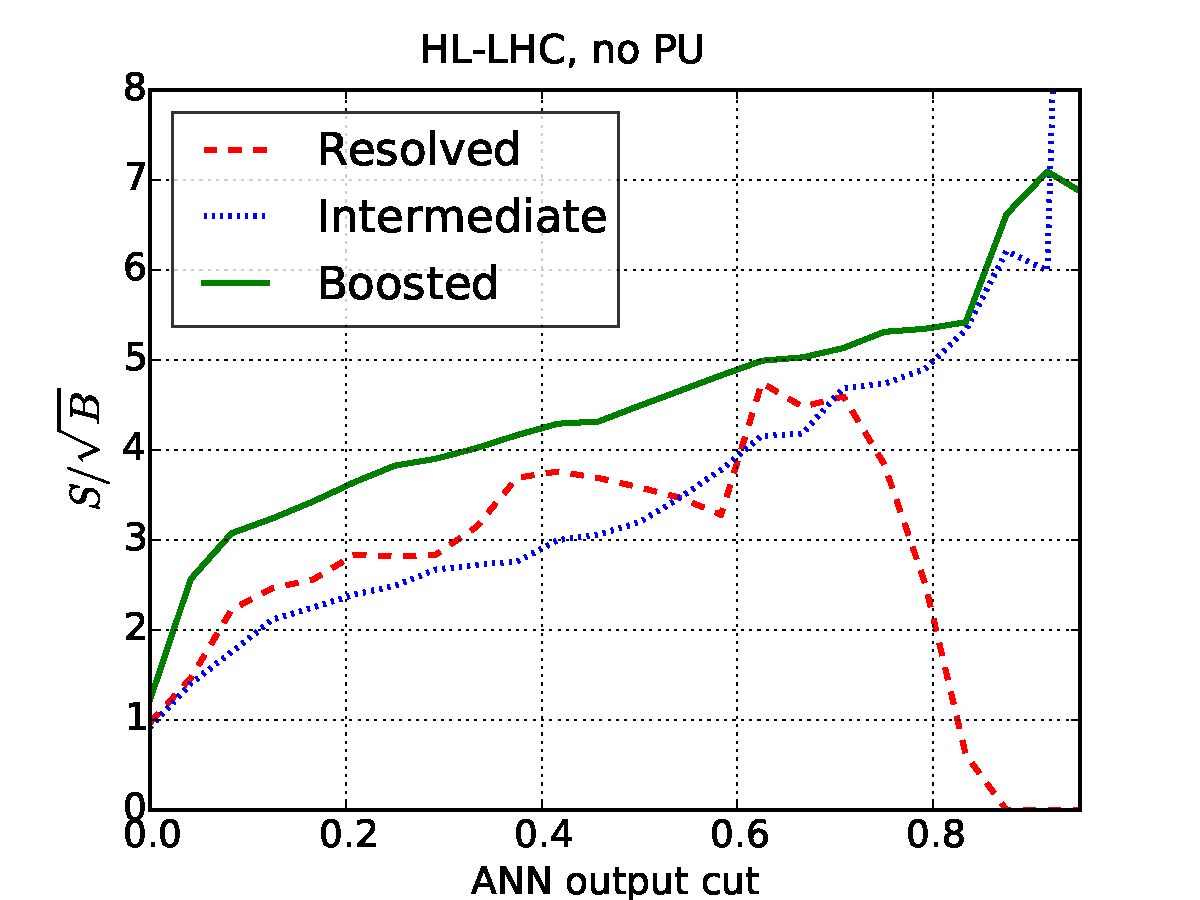
\includegraphics[width=0.48\textwidth]{plots/ssb_noPU.pdf}
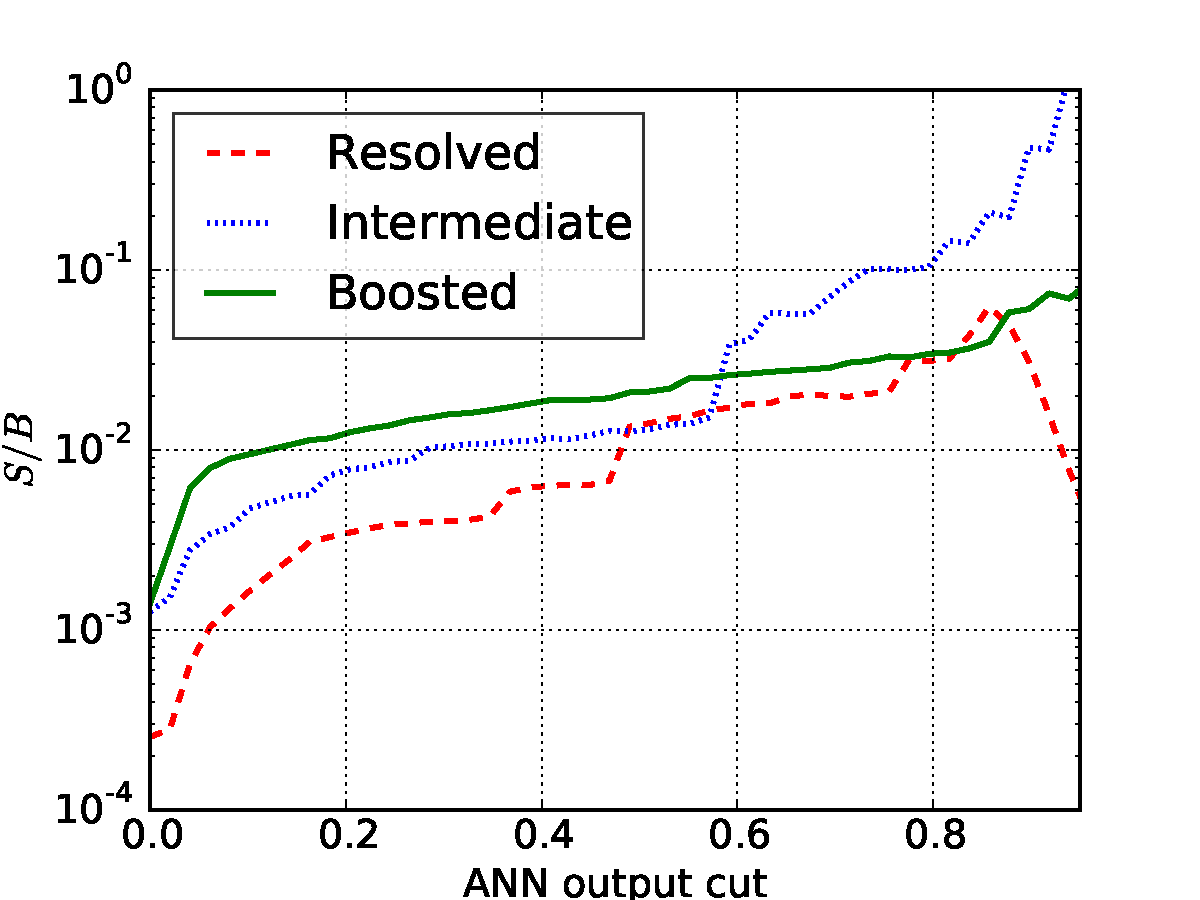
\includegraphics[width=0.48\textwidth]{plots/sb_noPU.pdf}
\caption{\small
  The values of the signal significance, $S/\sqrt{B}$, and of the
  signal over background ratio, $S/B$, for the boosted, intermediate
  and resolved categories as  function of the cut
  $y_{\rm cut}$ in the ANN output.
  %
  The $y_{\rm cut}=0$
  results are those at the end of the cut-based
  analysis.
}
\label{fig:sb_mva}
\end{center}
\end{figure}
%%%%%%%%%%%%%%%%%%%%%%%

The results for the signal significance $S/\sqrt{B}$ and
the signal over background ratio
$S/B$ as a function of $y_{\rm cut}$
for the three categories are
Fig.~\ref{fig:sb_mva}.
%
The values 
for $y_{\rm cut}=0$ correspond to those at
the end of the cut-based analysis.
%
We observe how in the three
 categories there is a marked  improvement in signal
significance as compared to the pre-MVA results.
%
We also observe a substantial enhancement in $S/B$, arising
from the background suppression achieved by the MVA, reaching
values of 1\%, 6\% and 3.5\% in the resolved,
intermediate and boosted categories.
%
This improvement in $S/B$ is crucial to ensure the feasibility
of this measurement, since it allows systematic
uncertainties in the background determination to
be at the same level of a few percent level.

We now have all the
information needed to determine a suitable
value of the MVA output cut $y_{\rm cut}$ in each
of the three categories.
%
These values can be determined from the maximisation of $S/\sqrt{B}$,
ensuring that the number of signal events $N_{\rm ev}$
expected at the HL-LHC is not too small.
%
In  addition, we require
that the number of MC events used to define the signal
category (events with $y_i \ge y_{\rm cut}$)
is large enough to avoid the biases and statistical
fluctuations associated to a small training sample.
%
In Table~\ref{table:cutflowMVA} where we quote
the value of the optimal ANN output
cut in each category,
the number of signal and background events $N_{\rm ev}$ expected
at the HL-LHC as well as $S/\sqrt{B}$ and $S/B$.
%
For reference, we also include the results at the end of
the cut-based
analysis.
%

%%%%%%%%%%%%%%%%%%%%%%%%%%%%%%%%%%%%%%%%%%%%%%%%%%%%%%%%%%%%%%%%%%%%%%%%%%%%
%%%%%%%%%%%%%%%%%%%%%%%%%%%%%%%%%%%%%%%%%%%%%%%%%%%%%%%%%%%%%%%%%%%%%%%%%%%%
\begin{table}[t]
  \centering
  \begin{tabular}{|c|l|c|c|c|c|}
    \hline
    \multicolumn{6}{|c|}{No PU} \\
    \hline
    \hline
    Category  &   &  $N_{\rm ev}$ signal &  $N_{\rm ev}$ back  &  $S/\sqrt{B}$ & $S/B$ \\ 
    \hline
    \hline
    \multirow{2}{*}{Boosted} &  $y_{\rm cut}=0$  & 1070 & $7.6\cdot 10^5$  & 1.2  & $1.4\cdot 10^{-3}$  \\
    &  $y_{\rm cut}=0.82$ & 790  & $2.2\cdot 10^4$   & 5.4  & 0.034 \\
    \hline
    \hline
    \multirow{2}{*}{Intermediate} &  $y_{\rm cut}=0$  & 670   & $5.3\cdot 10^5$
    & 0.9 & $1.2\cdot 10^{-3}$ \\
    &  $y_{\rm cut}=0.80$ & 360  & $5.5\cdot 10^3$  & 4.8 & 0.06\\
    \hline
    \hline
      \multirow{2}{*}{Resolved} &  $y_{\rm cut}=0$  & 3700 &  $1.5\cdot 10^{7}$ &  1.0 &$3\cdot 10^{-4}$ \\
    &  $y_{\rm cut}=0.65$ & 1300  & $8.3\cdot 10^{4}$ & 4.5 & 0.01 \\
    \hline
      \end{tabular}
  \caption{\small Post-MVA results, for the optimal value of the
    ANN discriminant $y_{\rm cut}$ in the three categories, compared with the
    corresponding
    pre-MVA results $y_{\rm cut}=0$.
    %
    we quote the number of signal and
    background events
    at the HL-LHC with $\mathcal{L}=3$ ab$^{-1}$,
    the signal significance $S/\sqrt{B}$ and
    the signal over background ratio $S/B$.
    %
    The pre-MVA results ($y_{\rm cut}=0$) corresponds to row C2 in
    Table~\ref{tab:cutflow_noPU_1}.
    \label{table:cutflowMVA}
  }
\end{table}
%%%%%%%%%%%%%%%%%%%%%%%%%%%%%%%%%%%%%%%%%%%%%%%%%%%%%%%%%%%%%%%%%%%%%%%%%%%%
%%%%%%%%%%%%%%%%%%%%%%%%%%%%%%%%%%%%%%%%%%%%%%%%%%%%%%%%%%%%%%%%%%%%%%%%%%%%




From Table~\ref{table:cutflowMVA} we see that
after we apply the MVA
the signal significance in the boosted category increases
from 1.2 to 5.4, with $S/B$ increasing from $0.14\%$ to $3.4\%$,
with almost 800 signal events expected at the HL-LHC.
%
For the intermediate and resolved category, $S/\sqrt{B}$
increases from 0.9 and 1.0 to 4.8 and 4.5, with
the signal over background ratio raising from
$0.12\%$ and $0.03\%$ to 6\% and 1\$, respectively.
%
The overall combined significance is thus $S\sqrt{B}\simeq 8$,
well above the threshold for discovery.
%
These remarkable results are however subject to a justified
criticism:
the HL-LHC will be a high-PU environment,
which will affect the description of the various
kinematical distributions used as input to the MVA.
%
Therefore, next we quantify the robustness of the
results summarized Table~\ref{fig:sb_mva}
in a realistic high-PU environment.

\subsection{Impact of PU in the MVA}

In this section we study how the MVA results are modified when
signal and background events are embedded in a high-PU environment.
%
The simulation of PU and the corresponding subtraction with
{\tt SoftKiller} have been performed as described
in Sect.~\ref{sec:pileup}.
%
The cut-based analysis and the subsequent
MVA optimization have been performed using exactly the same
settings as in the case without PU.
%
In Table~\ref{table:cutflowMVA_PU} we provide the results
  at the end of the cut-based analysis,
  for the case with $\la n_{\rm PU}\ra=80$ with SK
  subtraction.
%
It is clear that the pre-MVA 
signal significance has been degraded
as compared to the case without PU.
%
We now find values for $S/\sqrt{B}$ of 0.25, 0.15 and 0.31, in the resolved,
intermediate and boosted categories, respectively, to be compared
with the corresponding values without PU, namely 1.0, 0.9 and 1.0,
see Table~\ref{table:cutflowMVA}. 
%

Subsequently to 
 the cut-based analysis, the signal and background
 MC events in the case of PU satisfying all selection cuts
  are used to re-train the MVA.
%
In Table~\ref{table:cutflowMVA_PU}
we also provide  the number of signal and
    background events expected
    at the HL-LHC with $\mathcal{L}=3$ ab$^{-1}$,
    as well as the
    corresponding values for $S/\sqrt{B}$ and $S/B$,
    for both the cut-based analysis (corresponding
    to $y_{\rm cut}=0$) and after the
    optimal MVA cut.
    %
    From Table~\ref{table:cutflowMVA_PU} we observe that, thanks
to the MVA, the signal significance and the
signal over background ratio is improved from 0.31 and $3\cdot 10^{-4}$
(0.25 and $10^{-4}$) up to 2.9 and 3.4\% (2.5 and 1.5\%)
in the boosted (resolved) category.
%
The intermediate category, on the other hand, exhibits a
significantly lower post-MVA value of $S/\sqrt{B}\simeq
1.1$.
%
We thus conclude that, as was already the case
without PU,
the boosted category is the most promising
one for the study of Higgs pair production in the $b\bar{b}b\bar{b}$
final state
at the HL-LHC, also for the case of a high-PU environment, but that
important information will also be obtained from
the resolved category, which has a comparable significance.


%%%%%%%%%%%%%%%%%%%%%%%%%%%%%%%%%%%%%%%%%%%%%%%%%%%%%%%%%%%%%%%%%%%%%%%%%%%%
%%%%%%%%%%%%%%%%%%%%%%%%%%%%%%%%%%%%%%%%%%%%%%%%%%%%%%%%%%%%%%%%%%%%%%%%%%%%
\begin{table}[t]
  \centering
  \begin{tabular}{|c|l|c|c|c|c|}
        \hline
     \multicolumn{6}{|c|}{$\la n_{\rm PU}\ra=80$+SK} \\
     \hline
         \hline
    Category  &   &  $N_{\rm ev}$ signal &  $N_{\rm ev}$ back  &  $S/\sqrt{B}$ & $S/B$ \\ 
    \hline
    \hline
    \multirow{2}{*}{Boosted} &  $y_{\rm cut}=0$  & 360   &  $1.4\cdot 10^6$ & 0.31   &
     $3\cdot 10^{-4}$  \\
    &  $y_{\rm cut}=0.82$ &  250 & 7300  & 2.9    & 0.034  \\
    \hline
    \hline
    \multirow{2}{*}{Intermediate} &  $y_{\rm cut}=0$  &  150  & $9\cdot 10^5$    & 0.15    &
     $2\cdot 10^{-4}$ \\
    &  $y_{\rm cut}=0.80$ & 50 & 2600  &  1.1   & 0.02 \\
    \hline
    \hline
    \multirow{2}{*}{Resolved} &  $y_{\rm cut}=0$  &  1100  & $8.5\cdot 10^6$
    & 0.25    &  $1.3\cdot 10^{-4}$  \\
    &  $y_{\rm cut}=0.65$ & 430  & $3\cdot 10^4$  &  2.5   & 0.015  \\
    \hline
      \end{tabular}
  \caption{\small Same as Table~\ref{table:cutflowMVA}, now for the case
    of PU+SK, with $\la n_{\rm PU}\ra=80$.
        \label{table:cutflowMVA_PU}
  }
\end{table}
%%%%%%%%%%%%%%%%%%%%%%%%%%%%%%%%%%%%%%%%%%%%%%%%%%%%%%%%%%%%%%%%%%%%%%%%%%%%
%%%%%%%%%%%%%%%%%%%%%%%%%%%%%%%%%%%%%%%%%%%%%%%%%%%%%%%%%%%%%%%%%%%%%%%%%%%%

Another important result from Table~\ref{table:cutflowMVA_PU} is that,
for the optimal MVA cut, the signal over background ratio
is 3.4\% (1.5\%)
in the boosted (resolved) categories.
%
This indicates that while this measurement is still highly challenging,
requiring a careful extraction of the QCD
background from the data, it is certainty within reach.
%
As in the case without PU, 
our analysis  points out that both
$S/B$ and $S/\sqrt{B}$ could be increased  by reducing the background component
that arises from the mis-identification of light and charm
jets as $b$-jets.

In Fig.~\ref{fig:nev2_PU}
we show the number of signal and background events that
are expected at the HL-LHC as a function of
$y_{\rm cut}$, as well as the corresponding ROC curve.
%
Comparing Figs.~\ref{fig:nev2} and~\ref{fig:nev2_PU}, we observe
that the intermediate category is substantially degraded once PU effects
are accounted for due to a sizable
reduction in the number of signal
events that are now classified in this category.
%
This shows that the selection criteria
of the intermediate category are less
resilient against PU contamination,
as opposed to the resolved and boosted selections.

%%%%%%%%%%%%%%%%%%%%%%%%%%%%%%%%%%%%%%%%%%%%%
\begin{figure}[t]
  \begin{center}
    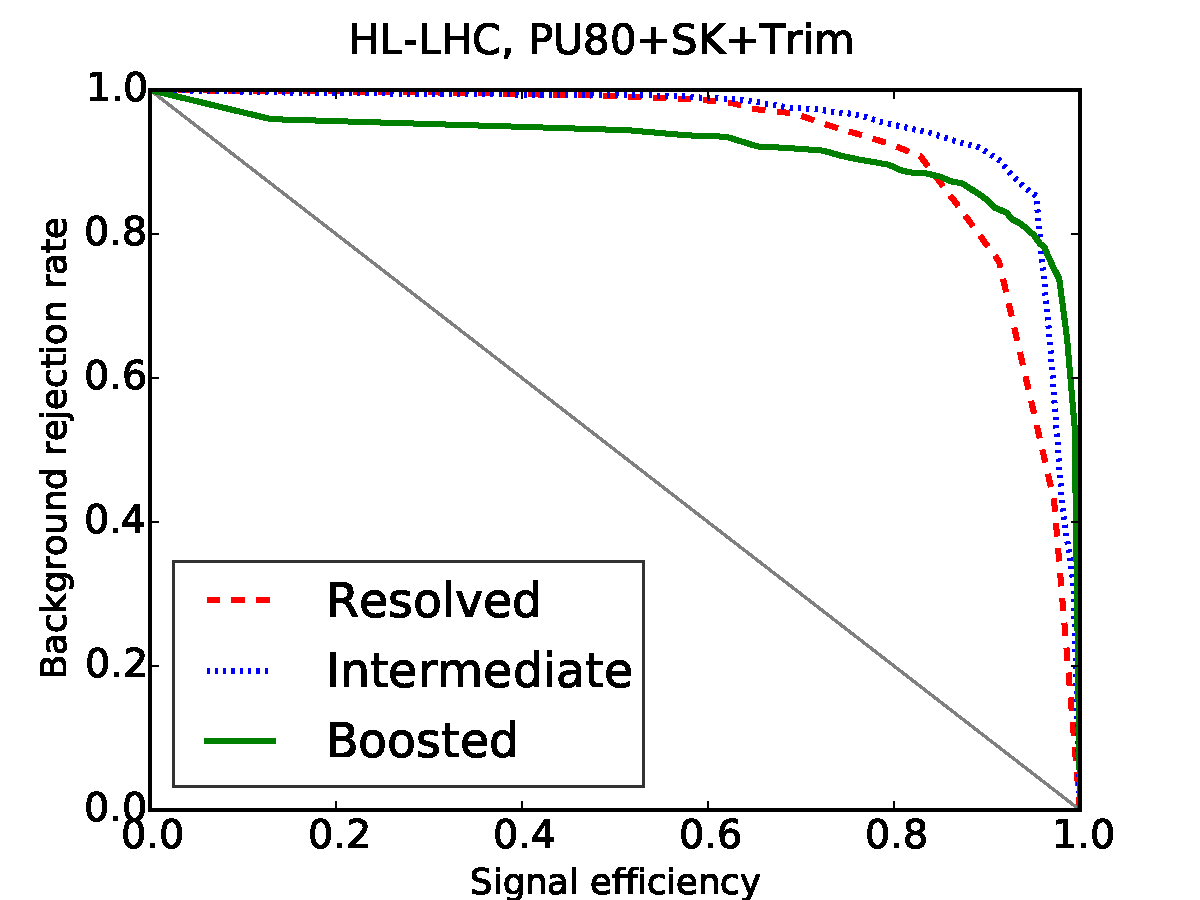
\includegraphics[width=0.49\textwidth]{plots/roc_SKPU80.pdf}
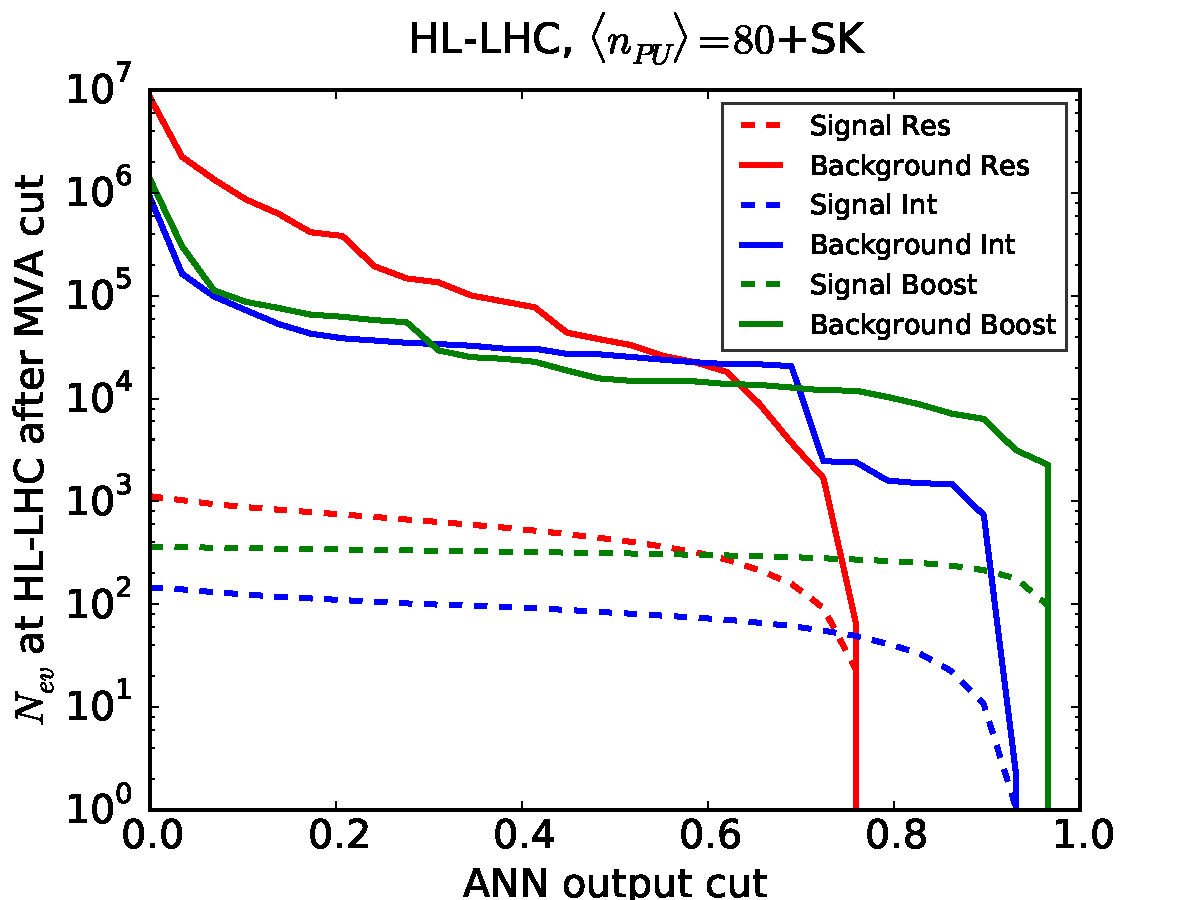
\includegraphics[width=0.49\textwidth]{plots/nev2_SKPU80.pdf}
\caption{\small Same as Fig.~\ref{fig:nev2} in the
case of events with PU, for
$\la n_{\rm PU}\ra=80$ using
{\tt SoftKiller} for PU subtraction.
}
\label{fig:nev2_PU}
\end{center}
\end{figure}
%%%%%%%%%%%%%%%%%%%%%%%%%%%%%%%%%%%%%


In Fig.~\ref{fig:sb_mva_PU} we show the signal significance,
$S/\sqrt{B}$, and the signal over background ratio,
$S/B$, accounting now for the effects of PU.
%
The corresponding results in the case without PU were shown in
Fig.~\ref{fig:sb_mva}.
%
As can be seen, the MVA-driven enhancement is robust in the
presence of PU.
%
While
there is some degradation as compared to the case
without PU,
it is still possible to
achieve a signal significance of
around $S/\sqrt{B}$ between 2.5 and 3.0 (depending on the
specific choice of $y_{\rm cut}$)
separately for the boosted and resolved
categories.
%
On the other hand, the intermediate category is now marginal.
%
We conclude that the qualitative conclusions drawn
in the case without PU also hold when the analysis
is performed in a high-PU environment.
%
Since no specific effort has been performed to
optimize PU subtraction, for instance by tuning the value
of the patch length $a$ in {\tt SoftKiller}, we believe that
there could be still room for further  improvement.


%%%%%%%%%%%%%%%%%%%%%%%%%%%%%%%%%%%%%%%%%%%%%%%%%%%%
%%%%%%%%%%%%%%%%%%%%%%%%%%%%%%%%%%%%%%%%%%%%%%%%%%%%
\begin{figure}[t]
\begin{center}
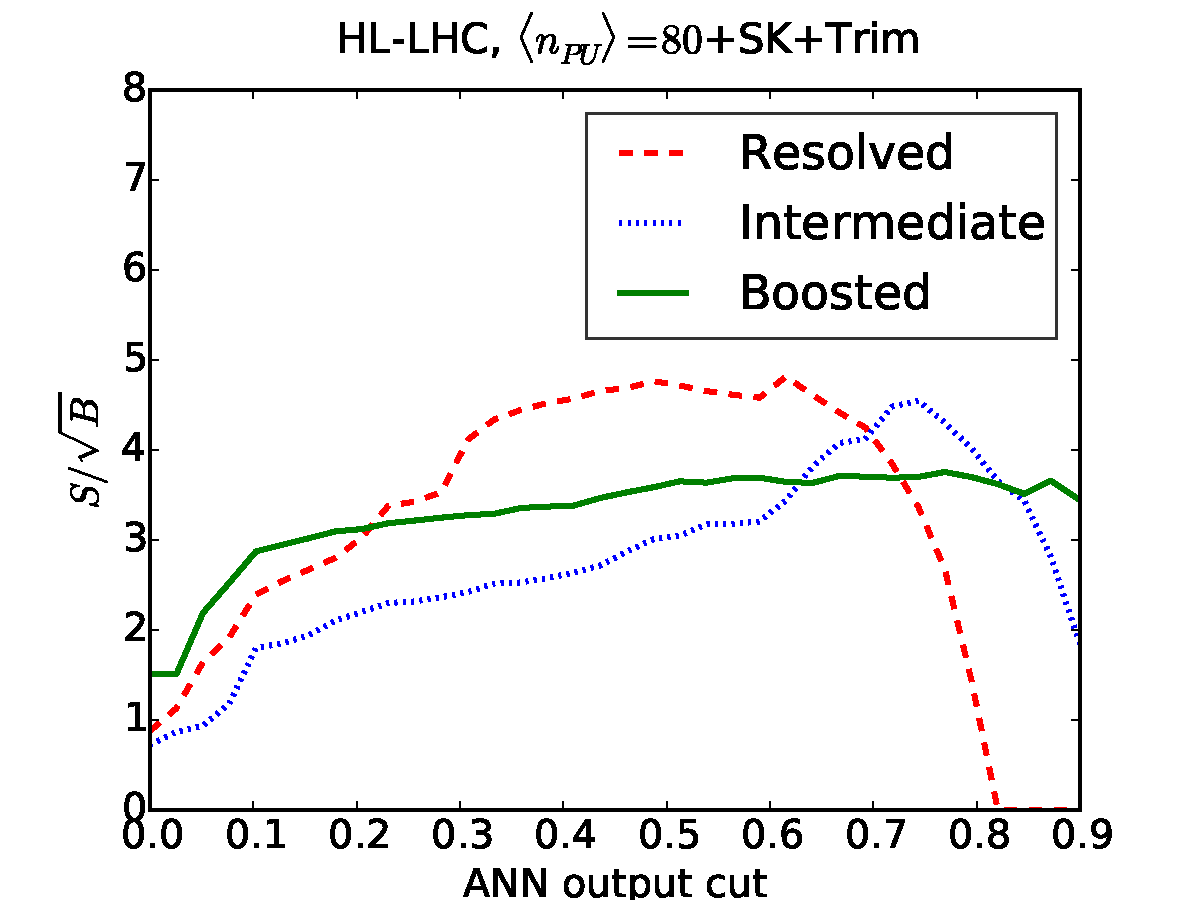
\includegraphics[width=0.48\textwidth]{plots/ssb_SKPU80.pdf}
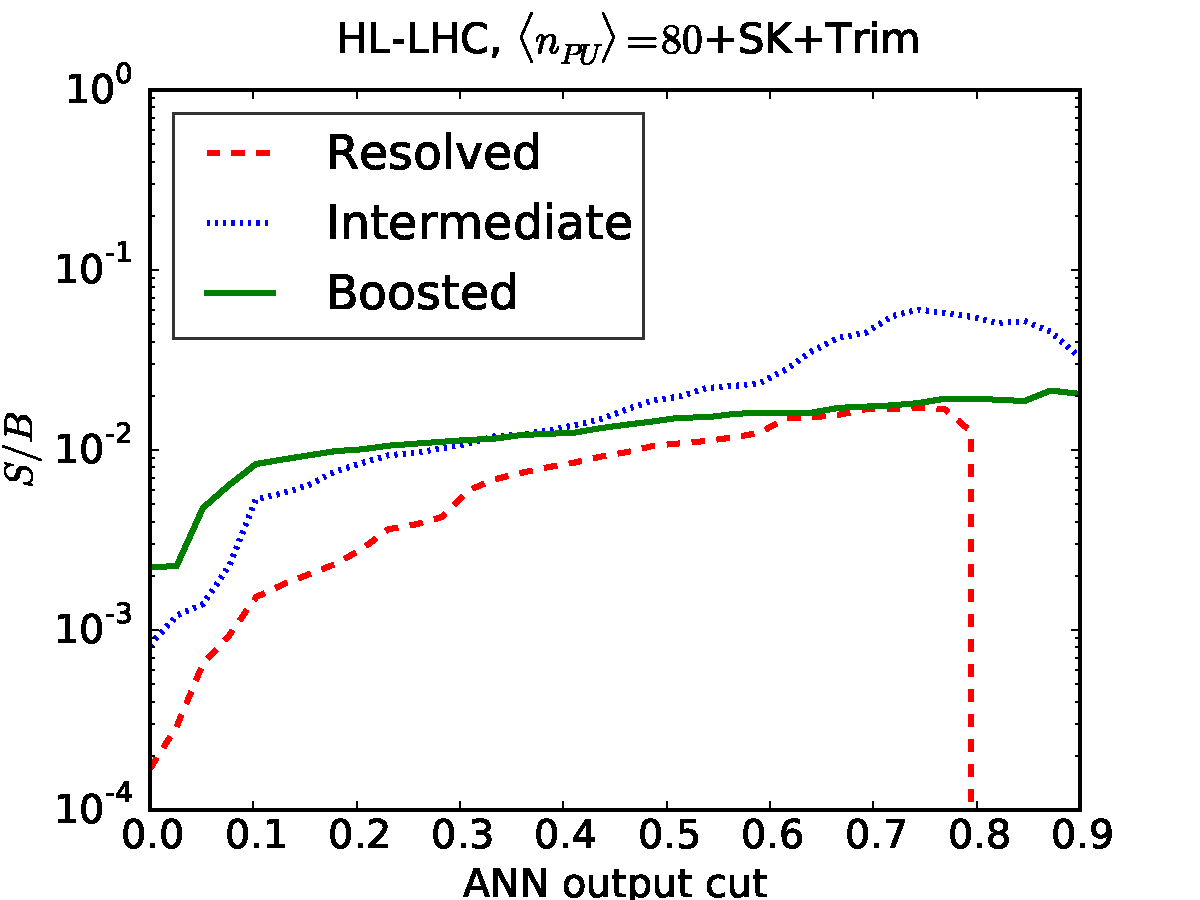
\includegraphics[width=0.48\textwidth]{plots/sb_SKPU80.pdf}
\caption{\small 
Same as Fig.~\ref{fig:sb_mva} in the
case of events with PU, for
$\la n_{\rm PU}\ra=80$
using
{\tt SoftKiller} for PU subtraction.
}
\label{fig:sb_mva_PU}
\end{center}
\end{figure}
%%%%%%%%%%%%%%%%%%%%%%%

It is useful to quantify which of the input variables
to the MVA carry the highest discrimination power
in the case of PU,
and compare this with the corresponding
results without PU, by means of
Eq.~(\ref{eq:totweight}).
%
The 
results for the resolved and boosted categories are shown
on Fig.~\ref{fig:nnweights_PU}.
%
As we can see by comparing with Fig.~\ref{fig:nnweights}, 
in the boosted category, the discrimination power of the invariant
mass of Higgs candidates is decreased, while
that of  substructure
variables such as $C_2^{(\beta)}$ and
$D^{(\beta)}_2$ is conversely
increased.
%
In addition, also the $p_T$ distributions of the AKT03
subjets within the large-$R$
jets carry important information.
%
In the case of the resolved category,  the highest
values of the ANN weights without PU
were found for the $p_T$ of the 
Higgs candidates and their invariant masses, as well
as the for invariant mass of the di-Higgs system
and the $p_T$ of the small-$R$ jets.
%
As we can see in Fig.~\ref{fig:nnweights_PU},
this is the case also with PU.

%%%%%%%%%%%%%%%%%%%%%%%%
\begin{figure}[t]
\begin{center}
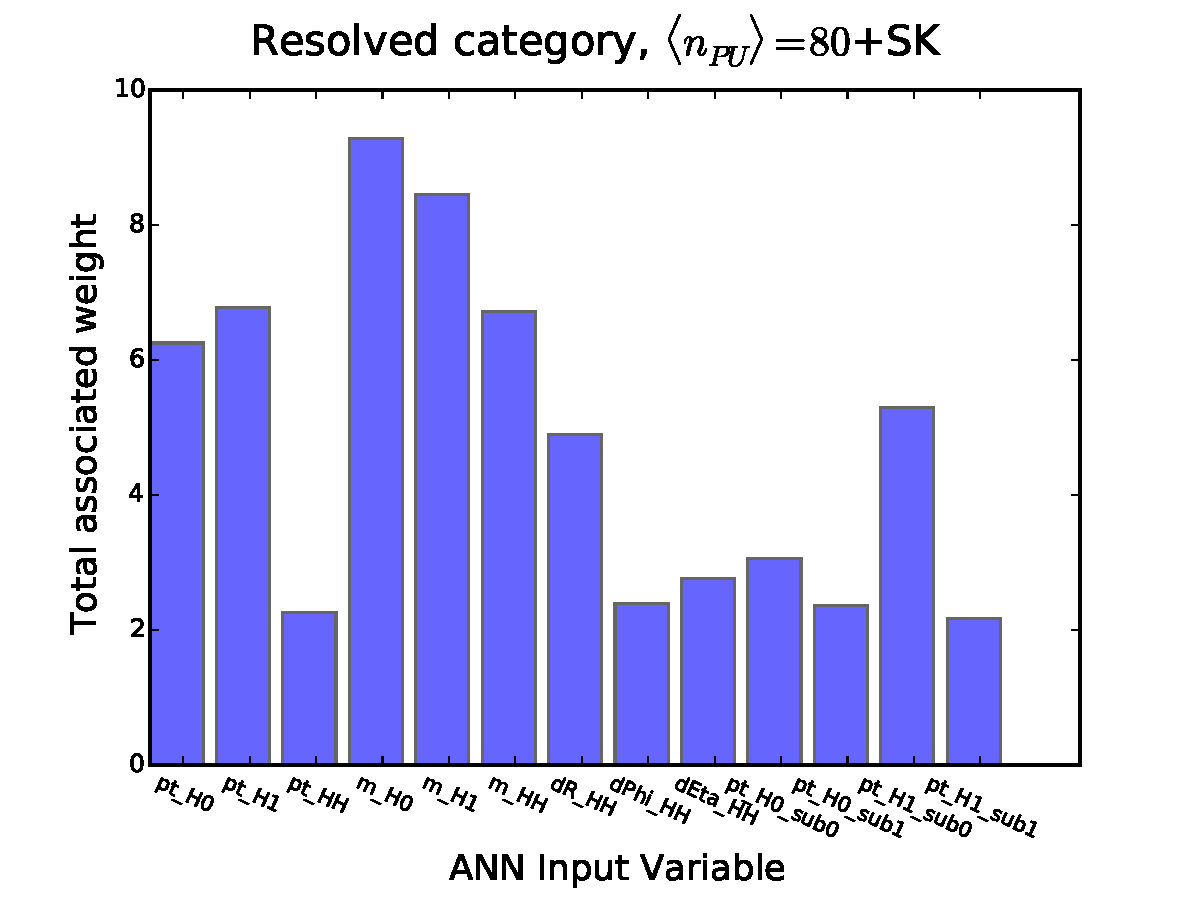
\includegraphics[width=0.49\textwidth]{plots/res_wgthist_SKPU80.pdf}
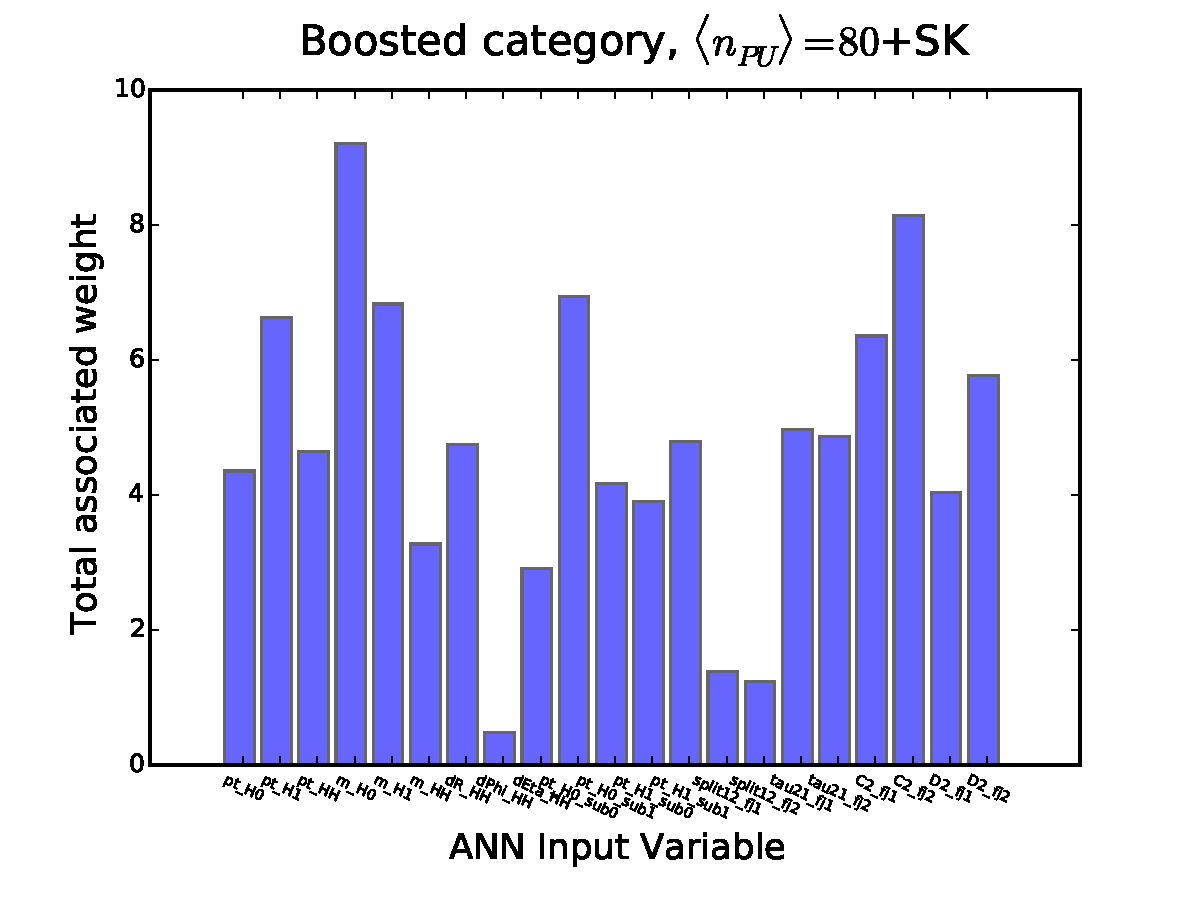
\includegraphics[width=0.49\textwidth]{plots/bst_wgthist_SKPU80.pdf}
\vspace{-0.5cm}
\caption{\small
Same as Fig.~\ref{fig:nnweights} in the
case of events with PU, for
$\la n_{\rm PU}\ra=80$
using
{\tt SoftKiller} for PU subtraction.
}
\label{fig:nnweights_PU}
\end{center}
\end{figure}
%%%%%%%%%%%%%%%%%%%%%%%


Combining the three categories, resolved,
intermediate and boosted, we determine the overall signal
significance, finding
\be
\lp \frac{S}{\sqrt{B}}\rp_{\rm tot} \simeq 4.0~(1.3) \, ,\quad
\mathcal{L}=3000~(300)\,{\rm fb}^{-1}\, .
\ee
%
We thus conclude that the measurement of
Higgs pair production in the $b\bar{b}b\bar{b}$ final state at the HL-LHC
should be 
well above the threshold for evidence.
%
On the other hand, such measurement seems to be out of reach
for the total integrated luminosity expected by the end of Run II.

In Table~\ref{table:cutflowMVA_fakes} we compare,
after the MVA is applied,
the total
number of background events, $N_{\rm ev}^{\rm tot}$,
    expected at the HL-LHC, with
     $N_{\rm ev}^{\rm 4b}$, the corresponding number
    from the QCD $4b$ component, in the cases with and without
    PU.
    %
    The MVA has been trained to the total background sample,
    though differences
    in the kinematic distributions of the $4b$ and $2b2j$ processes are small,
    see Fig.~\ref{fig:histoBack}.
    %
    The major improvement of eliminating the contamination
    of light and charm jet mis-identification is for the boosted and resolved categories.
%
    In the case of PU+SK, combining the three categories but assuming that
    the only relevant background is the irreducible QCD $4b$ component,
    we obtain
    \be
\lp \frac{S}{\sqrt{B_{\rm 4b}}}\rp_{\rm tot} \simeq 5.3~(1.8) \, ,\quad
\mathcal{L}=3000~(300)\,{\rm fb}^{-1}\, ,
\ee
Therefore, a discovery of Higgs pair production at the
HL-LHC might be possible if the
mis-identification of light and charm jets as
$b$-jets can be  reduced.
%
With these assumptions, and provided
the signal efficiency can be further enhanced,
this measurement might even be feasible
by the end of Run II.
%



%%%%%%%%%%%%%%%%%%%%%%%%%%%%%%%%%%%%%%%%%%%%%%%%%%%%%%%%%%%%%%%%%%%%%%%%%%%%
%%%%%%%%%%%%%%%%%%%%%%%%%%%%%%%%%%%%%%%%%%%%%%%%%%%%%%%%%%%%%%%%%%%%%%%%%%%%
\begin{table}[h]
  \centering
  \small
  \begin{tabular}{|c|c|c|c||c|c||c|c|}
        \hline
        Category  &    &  $N_{\rm ev}^{\rm tot}$  &  $N_{\rm ev}^{\rm 4b}$   &
        $S/\sqrt{B_{\rm tot}}$ & $S/\sqrt{B_{\rm 4b}}$  
        &  $S/B_{\rm tot}$ & $S/B_{\rm 4b}$\\ 
    \hline
    \hline
    \multirow{2}{*}{Boosted} &  no PU  & $2.2\cdot 10^4$  & $1.5\cdot 10^4$     & 
      5.4 &  6.5 & 0.034 & 0.05 \\
    & PU+SK & 7300  &  500  &  2.9  & 3.6 &  0.034 & 0.04 \\
    \hline
    \hline
    \multirow{2}{*}{Intermediate} &  no PU   & 4500  & 2000    &
    4.8  &  5.3 &  0.06  &  0.08 \\
    & PU+SK  & 2600   &  1500  & 1.1  & 1.2 & 0.02 & 0.03 \\
    \hline
    \hline
    \multirow{2}{*}{Resolved} &   no PU  & $8\cdot 10^4$   &
    $4.5\cdot 10^4$
    & 4.5  & 6.6  & 0.01 & 0.03 \\
    & PU+SK  &  $3\cdot 10^4$   &   $1.3\cdot 10^4$ & 2.5    & 3.7  & 0.015 & 0.03 \\
    \hline
      \end{tabular}
  \caption{\small Post-MVA number of total background events, $N_{\rm ev}^{\rm tot}$,
    expected at the HL-LHC, compared
    with $N_{\rm ev}^{\rm 4b}$,
    the number of QCD $4b$ background events.
    %
    We also indicate the corresponding signal significance and signal over background
    ratios.
        \label{table:cutflowMVA_fakes}
  }
\end{table}
%%%%%%%%%%%%%%%%%%%%%%%%%%%%%%%%%%%%%%%%%%%%%%%%%%%%%%%%%%%%%%%%%%%%%%%%%%%%
%%%%%%%%%%%%%%%%%%%%%%%%%%%%%%%%%%%%%%%%%%%%%%%%%%%%%%%%%%%%%%%%%%%%%%%%%%%%




%%%%%%%%%%%%%%%%%%%%%%%%%%%%%%%%%%%%%%%%%%%%%%%%%%%%%%%%%%%%%%%%%%%%%%%%%%%%%%%%
%%%%%%%%%%%%%%%%%%%%%%%%%%%%%%%%%%%%%%%%%%%%%%%%%%%%%%%%%%%%%%%%%%%%%%%%%%%%%%%%
%%%%%%%%%%%%%%%%%%%%%%%%%%%%%%%%%%%%%%%%%%%%%%%%%%%%%%%%%%%%%%%%%%%%%%%%%%%%%%%%
%%%%%%%%%%%%%%%%%%%%%%%%%%%%%%%%%%%%%%%%%%%%%%%%%%%%%%%%%%%%%%%%%%%%%%%%%%%%%%%%
%%%%%%%%%%%%%%%%%%%%%%%%%%%%%%%%%%%%%%%%%%%%%%%%%%%%%%%%%%%%%%%%%%%%%%%%%%%%%%%%
